زبان داده‌شده روی $\Sigma = \{0,1\}$ این است:

\[
L = \bigl\{\, w \in \Sigma^* \mid w \in \Sigma^* 101 \ \land\ |w|_0 \iequiv{3} 2 \,\bigr\}.
\]
یعنی $w$ باید هم‌زمان با الگوی $101$ به‌پایان برسد و تعداد نمادهای $0$ در $w$ باقیماندهٔ $2$ بر پیمانهٔ $3$ داشته باشد.
این زبان اشتراک دو زبان منظم است؛ پس دو DFA مجزا را ترکیب می‌کنیم و یک DFA یکتا به‌دست می‌آید.

ماشین نهایی با ساخت ضرب دو DFA (ردیابی پسوند $101$ و شمارش باقی‌مانده) ساخته می‌شود.
در جدول زیر هر حالت به‌صورت $[\sigma,j]$ نوشته شده است: $\sigma$ بلندترین پسوند مسیر است که پیشوند $101$ باشد ($\sigma\in\{\varepsilon,1,10,101\}$) و $j\in\{0,1,2\}$ باقیماندهٔ تعداد نماد $0$ پس از خواندن همان پیشوند است.
\begin{center}
\begin{tabular}{|c|c|c|}
\hline
حالت فعلی & با ۰ به & با ۱ به \\
\hline
$[\varepsilon,0]$ & $[\varepsilon,1]$ & $[1,0]$ \\
$[\varepsilon,1]$ & $[\varepsilon,2]$ & $[1,1]$ \\
$[\varepsilon,2]$ & $[\varepsilon,0]$ & $[1,2]$ \\
\hline
$[1,0]$ & $[10,1]$ & $[1,0]$ \\
$[1,1]$ & $[10,2]$ & $[1,1]$ \\
$[1,2]$ & $[10,0]$ & $[1,2]$ \\
\hline
$[10,0]$ & $[\varepsilon,1]$ & $[101,0]$ \\
$[10,1]$ & $[\varepsilon,2]$ & $[101,1]$ \\
$[10,2]$ & $[\varepsilon,0]$ & $[101,2]$ \\
\hline
$[101,0]$ & $[10,1]$ & $[1,0]$ \\
$[101,1]$ & $[10,2]$ & $[1,1]$ \\
$[101,2]$ & $[10,0]$ & $[1,2]$ \\
\hline
\end{tabular}
\end{center}
تنها حالت پذیرش $[101,2]$ است.

\begin{center}
    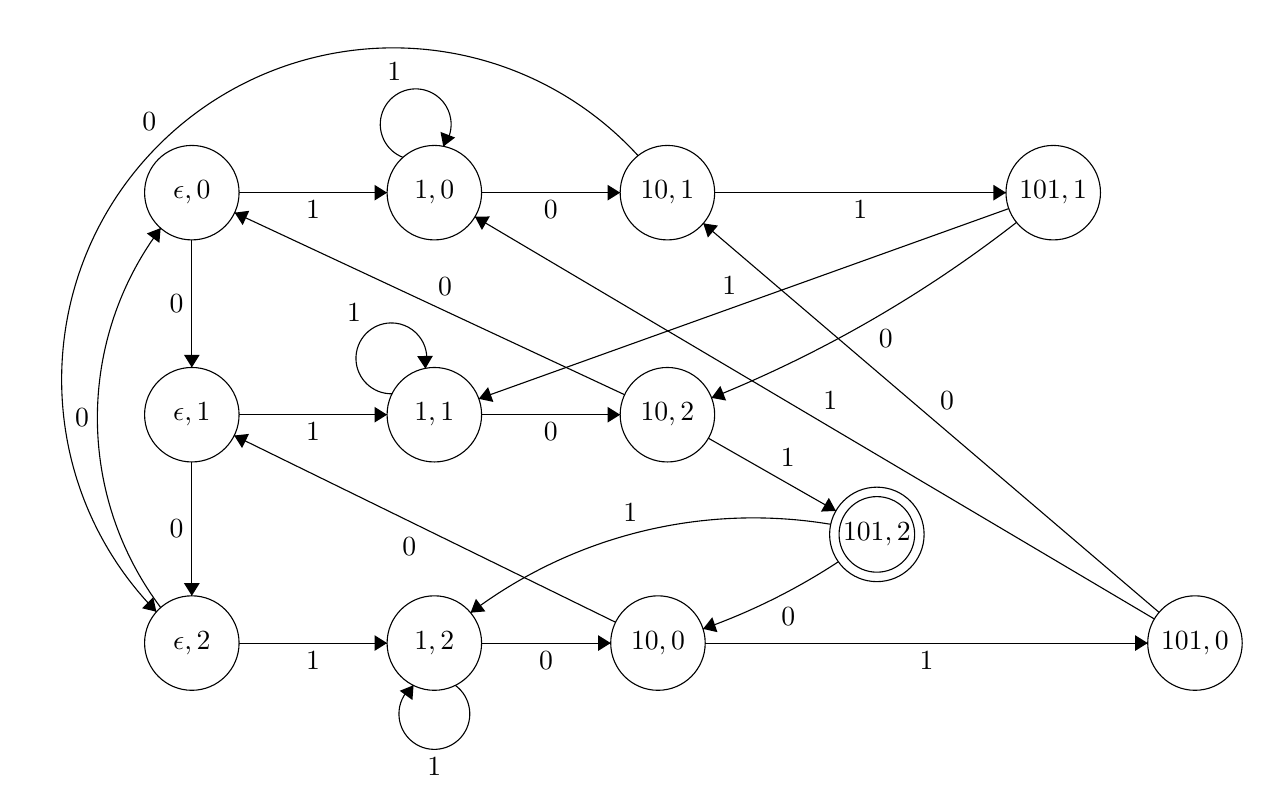
\begin{tikzpicture}[scale=0.2]
    \tikzstyle{every node}+=[inner sep=0pt]
    \draw [black] (12.4,-15.2) circle (3);
    \draw (12.4,-15.2) node {$\epsilon,0$};
    \draw [black] (12.4,-29.3) circle (3);
    \draw (12.4,-29.3) node {$\epsilon,1$};
    \draw [black] (12.4,-43.8) circle (3);
    \draw (12.4,-43.8) node {$\epsilon,2$};
    \draw [black] (27.8,-15.2) circle (3);
    \draw (27.8,-15.2) node {$1,0$};
    \draw [black] (27.8,-29.3) circle (3);
    \draw (27.8,-29.3) node {$1,1$};
    \draw [black] (27.8,-43.8) circle (3);
    \draw (27.8,-43.8) node {$1,2$};
    \draw [black] (42,-43.8) circle (3);
    \draw (42,-43.8) node {$10,0$};
    \draw [black] (42.6,-15.2) circle (3);
    \draw (42.6,-15.2) node {$10,1$};
    \draw [black] (42.6,-29.3) circle (3);
    \draw (42.6,-29.3) node {$10,2$};
    \draw [black] (76.1,-43.8) circle (3);
    \draw (76.1,-43.8) node {$101,0$};
    \draw [black] (67.1,-15.2) circle (3);
    \draw (67.1,-15.2) node {$101,1$};
    \draw [black] (55.9,-36.9) circle (3);
    \draw (55.9,-36.9) node {$101,2$};
    \draw [black] (55.9,-36.9) circle (2.4);
    \draw [black] (12.4,-18.2) -- (12.4,-26.3);
    \fill [black] (12.4,-26.3) -- (12.9,-25.5) -- (11.9,-25.5);
    \draw (11.9,-22.25) node [left] {$0$};
    \draw [black] (15.4,-15.2) -- (24.8,-15.2);
    \fill [black] (24.8,-15.2) -- (24,-14.7) -- (24,-15.7);
    \draw (20.1,-15.7) node [below] {$1$};
    \draw [black] (12.4,-32.3) -- (12.4,-40.8);
    \fill [black] (12.4,-40.8) -- (12.9,-40) -- (11.9,-40);
    \draw (11.9,-36.55) node [left] {$0$};
    \draw [black] (15.4,-29.3) -- (24.8,-29.3);
    \fill [black] (24.8,-29.3) -- (24,-28.8) -- (24,-29.8);
    \draw (20.1,-29.8) node [below] {$1$};
    \draw [black] (10.425,-41.546) arc (-143.06153:-216.93847:20.044);
    \fill [black] (10.42,-17.45) -- (9.54,-17.79) -- (10.34,-18.39);
    \draw (5.9,-29.5) node [left] {$0$};
    \draw [black] (15.4,-43.8) -- (24.8,-43.8);
    \fill [black] (24.8,-43.8) -- (24,-43.3) -- (24,-44.3);
    \draw (20.1,-44.3) node [below] {$1$};
    \draw [black] (30.8,-15.2) -- (39.6,-15.2);
    \fill [black] (39.6,-15.2) -- (38.8,-14.7) -- (38.8,-15.7);
    \draw (35.2,-15.7) node [below] {$0$};
    \draw [black] (25.819,-12.963) arc (249.25512:-38.74488:2.25);
    \draw (25.25,-8.13) node [above] {$1$};
    \fill [black] (28.37,-12.27) -- (29.12,-11.7) -- (28.19,-11.34);
    \draw [black] (30.8,-29.3) -- (39.6,-29.3);
    \fill [black] (39.6,-29.3) -- (38.8,-28.8) -- (38.8,-29.8);
    \draw (35.2,-29.8) node [below] {$0$};
    \draw [black] (25.124,-27.97) arc (271.3118:-16.6882:2.25);
    \draw (22.7,-23.44) node [above] {$1$};
    \fill [black] (27.23,-26.37) -- (27.71,-25.56) -- (26.71,-25.58);
    \draw [black] (30.8,-43.8) -- (39,-43.8);
    \fill [black] (39,-43.8) -- (38.2,-43.3) -- (38.2,-44.3);
    \draw (34.9,-44.3) node [below] {$0$};
    \draw [black] (29.123,-46.48) arc (54:-234:2.25);
    \draw (27.8,-51.05) node [below] {$1$};
    \fill [black] (26.48,-46.48) -- (25.6,-46.83) -- (26.41,-47.42);
    \draw [black] (39.31,-42.48) -- (15.09,-30.62);
    \fill [black] (15.09,-30.62) -- (15.59,-31.42) -- (16.03,-30.52);
    \draw (26.21,-37.06) node [below] {$0$};
    \draw [black] (45,-43.8) -- (73.1,-43.8);
    \fill [black] (73.1,-43.8) -- (72.3,-43.3) -- (72.3,-44.3);
    \draw (59.05,-44.3) node [below] {$1$};
    \draw [black] (10.155,-41.814) arc (-135.56981:-317.54756:21.065);
    \fill [black] (10.15,-41.81) -- (9.95,-40.89) -- (9.24,-41.59);
    \draw (9.7,-11.29) node [above] {$0$};
    \draw [black] (45.6,-15.2) -- (64.1,-15.2);
    \fill [black] (64.1,-15.2) -- (63.3,-14.7) -- (63.3,-15.7);
    \draw (54.85,-15.7) node [below] {$1$};
    \draw [black] (39.88,-28.03) -- (15.12,-16.47);
    \fill [black] (15.12,-16.47) -- (15.63,-17.26) -- (16.05,-16.35);
    \draw (28.48,-21.74) node [above] {$0$};
    \draw [black] (45.2,-30.79) -- (53.3,-35.41);
    \fill [black] (53.3,-35.41) -- (52.85,-34.58) -- (52.35,-35.45);
    \draw (50.25,-32.6) node [above] {$1$};
    \draw [black] (73.82,-41.85) -- (44.88,-17.15);
    \fill [black] (44.88,-17.15) -- (45.17,-18.05) -- (45.81,-17.29);
    \draw (60.36,-29.01) node [above] {$0$};
    \draw [black] (73.52,-42.27) -- (30.38,-16.73);
    \fill [black] (30.38,-16.73) -- (30.82,-17.57) -- (31.32,-16.71);
    \draw (52.95,-29) node [above] {$1$};
    \draw [black] (64.768,-17.087) arc (-52.08975:-68.06852:80.376);
    \fill [black] (45.4,-28.23) -- (46.33,-28.4) -- (45.96,-27.47);
    \draw (56.47,-23.84) node [below] {$0$};
    \draw [black] (64.28,-16.21) -- (30.62,-28.29);
    \fill [black] (30.62,-28.29) -- (31.55,-28.49) -- (31.21,-27.55);
    \draw (46.53,-21.72) node [above] {$1$};
    \draw [black] (53.455,-38.638) arc (-56.73529:-70.46484:40.132);
    \fill [black] (44.86,-42.9) -- (45.78,-43.11) -- (45.45,-42.16);
    \draw (50.28,-41.53) node [below] {$0$};
    \draw [black] (30.098,-41.874) arc (127.07993:80.5123:29.791);
    \fill [black] (30.1,-41.87) -- (31.04,-41.79) -- (30.44,-40.99);
    \draw (40.25,-36.14) node [above] {$1$};
    \end{tikzpicture}
    \end{center}
    